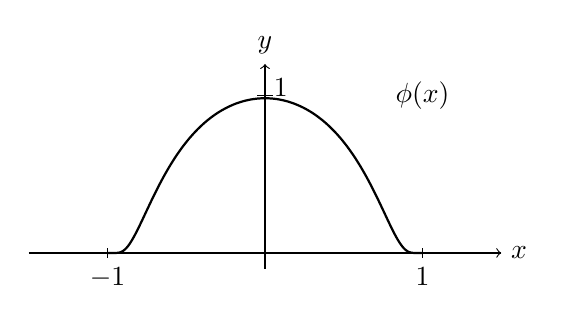
\begin{tikzpicture}[scale=2]

  % Ejes
  \draw[->] (-1.5,0) -- (1.5,0) node[right] {$x$};
  \draw[->] (0,-0.1) -- (0,1.2) node[above] {$y$};

  % Bump function
  \draw[
      domain=-0.999:0.999,
      samples=200,
      smooth,
      thick
  ]
  plot (\x,{2.67*exp(-1/(1-\x*\x))});
  
  % Parte cero
  \draw[thick] (-1.5,0) -- (-1,0);
  \draw[thick] (1,0) -- (1.5,0);
  
  % Marcas
  \draw (-1,0.03) -- (-1,-0.03) node[below] {$-1$};
  \draw (1,0.03) -- (1,-0.03) node[below] {$1$};
  \draw (-0.05,1) -- (0.05,1);
  \node at (0.1,1.05) {$1$};

  \node at (1,1) {$\phi(x)$};
\end{tikzpicture}

